\tikzset{every picture/.style={line width=0.75pt}} %set default line width to 0.75pt        

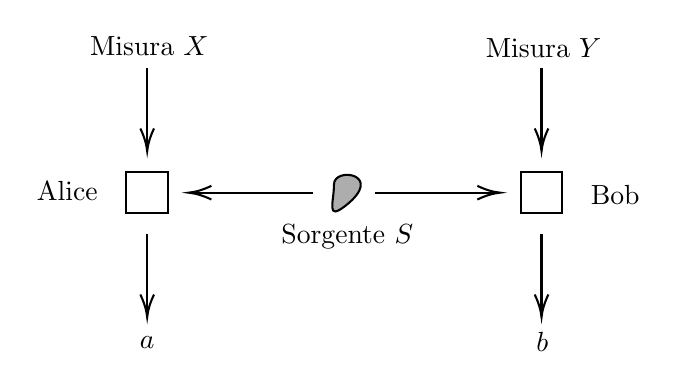
\begin{tikzpicture}[x=0.75pt,y=0.75pt,yscale=-1,xscale=1]
%uncomment if require: \path (0,300); %set diagram left start at 0, and has height of 300

%Shape: Square [id:dp9196862351413921] 
\draw   (260,120) -- (280,120) -- (280,140) -- (260,140) -- cycle ;
%Straight Lines [id:da17930112223236172] 
\draw    (270,70) -- (270,108) ;
\draw [shift={(270,110)}, rotate = 270] [color={rgb, 255:red, 0; green, 0; blue, 0 }  ][line width=0.75]    (10.93,-3.29) .. controls (6.95,-1.4) and (3.31,-0.3) .. (0,0) .. controls (3.31,0.3) and (6.95,1.4) .. (10.93,3.29)   ;

%Straight Lines [id:da47107310700179994] 
\draw    (270,150) -- (270,188) ;
\draw [shift={(270,190)}, rotate = 270] [color={rgb, 255:red, 0; green, 0; blue, 0 }  ][line width=0.75]    (10.93,-3.29) .. controls (6.95,-1.4) and (3.31,-0.3) .. (0,0) .. controls (3.31,0.3) and (6.95,1.4) .. (10.93,3.29)   ;

%Straight Lines [id:da3446633388248408] 
\draw    (350,130) -- (292,130) ;
\draw [shift={(290,130)}, rotate = 360] [color={rgb, 255:red, 0; green, 0; blue, 0 }  ][line width=0.75]    (10.93,-3.29) .. controls (6.95,-1.4) and (3.31,-0.3) .. (0,0) .. controls (3.31,0.3) and (6.95,1.4) .. (10.93,3.29)   ;

%Straight Lines [id:da822622270040033] 
\draw    (380,130) -- (438,130) ;
\draw [shift={(440,130)}, rotate = 180] [color={rgb, 255:red, 0; green, 0; blue, 0 }  ][line width=0.75]    (10.93,-3.29) .. controls (6.95,-1.4) and (3.31,-0.3) .. (0,0) .. controls (3.31,0.3) and (6.95,1.4) .. (10.93,3.29)   ;

%Shape: Square [id:dp7370593336819211] 
\draw   (450,120) -- (470,120) -- (470,140) -- (450,140) -- cycle ;
%Straight Lines [id:da5563468788997123] 
\draw    (460,70) -- (460,108) ;
\draw [shift={(460,110)}, rotate = 270] [color={rgb, 255:red, 0; green, 0; blue, 0 }  ][line width=0.75]    (10.93,-3.29) .. controls (6.95,-1.4) and (3.31,-0.3) .. (0,0) .. controls (3.31,0.3) and (6.95,1.4) .. (10.93,3.29)   ;

%Straight Lines [id:da6249187435301291] 
\draw    (460,150) -- (460,188) ;
\draw [shift={(460,190)}, rotate = 270] [color={rgb, 255:red, 0; green, 0; blue, 0 }  ][line width=0.75]    (10.93,-3.29) .. controls (6.95,-1.4) and (3.31,-0.3) .. (0,0) .. controls (3.31,0.3) and (6.95,1.4) .. (10.93,3.29)   ;

%Curve Lines [id:da7601728877448455] 
\draw [color={rgb, 255:red, 0; green, 0; blue, 0 }  ,draw opacity=1 ][fill={rgb, 255:red, 173; green, 173; blue, 173 }  ,fill opacity=1 ]   (365.5,136.33) .. controls (385,121) and (360,117.33) .. (360,126) .. controls (360,134.67) and (356,143.67) .. (365.5,136.33) -- cycle ;



% Text Node
\draw (231.5,129) node  [align=left] {Alice};
% Text Node
\draw (495.5,131) node  [align=left] {Bob};
% Text Node
\draw (366.4,151) node  [align=left] {Sorgente $\displaystyle S$};
% Text Node
\draw (271,59.5) node  [align=left] {Misura $\displaystyle X$};
% Text Node
\draw (461,60.5) node  [align=left] {Misura $\displaystyle Y$};
% Text Node
\draw (270,202) node   {$a$};
% Text Node
\draw (460.33,201.67) node   {$b$};


\end{tikzpicture}